\chapter{Estado del Arte}
Tomando en consideración lo amplio, en el sentido de las disciplinas a abarcar, de este trabajo de tesis, el resumen del estado del arte se llevará a cabo en cuatro secciones distintas. 

Primero se expondrá la problemática que nace debido a la turbulencia en las simulaciones multiescala. Luego se revisará la historia y la creciente utilización de la técnica de Simulación de Grandes Vórtices (de aquí en adelante \emph{Large Eddy Simulation} o LES) en la solución numérica de los modelos meteorológicos. Tercero, se verán las complicaciones y los desafíos que conlleva el realizar simulaciones de alta resolución en terreno complejo y los consensos internacionales tomados al respecto. Finalmente se mostrará el estado actual de la utilización de los métodos de asimilación de datos para el uso operacional en el contexto de las simulaciones atmosféricas y la capa límite planetaria.
\newpage
\section{Simulación Multiescala y Zona Gris}
Como ya se justificó en la introducción, la predicción atmosférica en zonas localizadas, en especial en aquellas con terreno irregular, es un tema de especial relevancia en las áreas del cambio climático, la contaminación ambiental y la industria energética. Actualmente las simulaciones climáticas regionales se realizan con una resolución de malla del orden de los kilómetros. Esto es, evidentemente, insuficiente para poder representar fehacientemente cualquier topografía compleja, y por lo tanto, insuficiente también para resolver los fenómenos meteorológicos asociados a esta.

Una manera de solucionar esto puede ser el eso de un escalamiento estadístico para llevar las soluciones a una malla mas fina, sin embargo, este acercamiento no contempla ni la física fundamental ni las no-linealidades, que son la característica mas importante del comportamiento de la atmósfera en su interacción con el terreno complejo. Su contraparte, el escalamiento dinámico, permite anidar mallas y resolver las leyes de conservación para resoluciones cada vez mas altas hasta lo que se desee resolver, teniendo como limitantes: el costo computacional, la precisión de las condiciones de borde y las parametrizaciones físicas que se incorporarán a las ecuaciones. Para este trabajo, es claro el beneficio que trae el utilizar el escalamiento dinámico como metodología para alcanzar simulaciones de alta resolución y por lo tanto ese es el acercamiento que se utilizará.

A modo de formar una explicación un poco mas formal y clara sobre lo que conlleva el realizar una simulación atmosférica multiescala, tomemos en consideración la Figura \ref{fig:02_escalas} para identificar las distintas escalas temporales y espaciales presentes en la atmósfera.

\begin{figure}[h!]
	\centering
	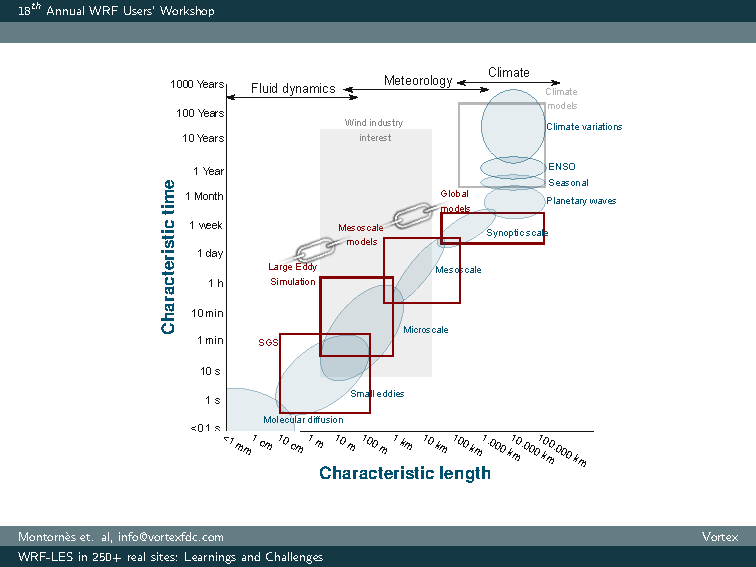
\includegraphics[width=0.8\linewidth,trim={2.6cm 1.4cm 1.5cm 0.8cm},clip]{Imagenes/02/escalas}
	\caption{Separación de escalas para la dinámica atmosférica.}
	\label{fig:02_escalas}
\end{figure}

La figura presenta tres aspectos claves de las simulaciones atmosféricas: las áreas del conocimiento involucradas, los fenómenos que resuelve cada área y las escalas asociadas a cada uno de estas.

Nos referimos a simulación multiescala cuando, a través de algún proceso de escalamiento y simulación numérica se resuelven simultáneamente distintas escalas espaciales y se representan correctamente sus fenómenos asociados.
 
Nos referimos, por otra parte, a escalamiento dinámico, cuando se resuelven escalas mas pequeñas usando como base una escala mas grande, la cual es usada como condición inicial y de contorno en un subdominio de un dominio general. De esta forma es posible tener resultados numéricos para la microescala partiendo desde una escala, por ejemplo, global. 

En el contexto del trabajo a realizar, las escalas temporales pertenecientes a las simulaciones serán del orden de los días, por lo tanto, los fenómenos que se engloban dentro de estas son una combinación entre fenómenos de microescala, mesoescala y escala sinóptica. El buen comportamiento del resultado de una simulación estará directamente relacionado con lo bien representado que estén cada uno de estos fenómenos dentro del modelo.

De manera general, el escalamiento dinámico funciona bien y solo incorpora al modelo un error de interpolación debido al traspaso de una malla mas gruesa a otra mas fina. Sin embargo, la presencia de la turbulencia a lo largo de todo el espectro de escalas complica el escalamiento desde la mesoescala hasta la microescala.

Para entender la complejidad asociada a la presencia de la turbulencia debido al escalamiento dinámico, hay que entender primero la manera en la que actúan las distintas fuerzas que controlan el movimiento atmosférico. Si se considera, por ejemplo, la fuerza de Coriolis que es el motor principal de los ciclones y anticiclones en los hemisferios, esta fuerza es relevante en escalas sinópticas y globales y si se quisiera resolver ecuaciones a un nivel de mesoescala, podrían ser válidamente despreciadas. Por otra parte, si se considera ahora, la disipación viscosa generada por el roce entre los distintos elementos diferenciales de aire, esta podría ser válidamente despreciada también en todas las escalas debido a que la viscosidad del aire es muy baja, sin embargo si se desea analizar la parte viscosa de la capa límite atmosférica, este término es fundamental y no podría despreciarse. 
 
Se concluye entonces que las distintas fuerzas que aparecen en las ecuaciones tienen un cierto rango de escalas propias donde contribuyen fuertemente al movimiento atmosférico. 

La turbulencia sin embargo\footnote{Probablemente le haga ruido al lector el hecho que hasta ahora no se ha presentado una definición formal de la turbulencia. Como esta requiere una descripción extensa se prefirió dejarla para el próximo capítulo.}, no funciona de la misma forma. Los vórtices de distintos tamaños que habitan en la atmósfera son igualmente importantes en términos de órdenes de magnitud para todas las escalas en las ecuaciones que se resuelven.

Cuando se modelan las grandes escalas (sinóptica, mesoescala), generalmente la resolución de malla horizontal es demasiado grande como para captar los vórtices y por lo tanto el efecto de estos en las ecuaciones queda filtrado numéricamente. Operacionalmente, esta operación de filtrado se revierte con la utilización de un esquema adecuado para parametrizar la turbulencia. En los modelos meteorológicos actuales este efecto generalmente queda confinado en la llamada \emph{parametrización de capa límite planetaria}, ya que el principal rol que cumple la turbulencia en estas escalas es la de transmitir la información que se genera a nivel de superficie terrestre a la atmósfera libre.

Cuando se modelan las pequeñas escalas, idealmente la resolución de malla horizontal va a bastar para captar de manera adecuada cierto espectro de los vórtices generados por el efecto de la turbulencia y por lo tanto se puede omitir la parametrización de capa límite. Es importante notar que si bien ahora se resuelven los vórtices grandes que provocan la mezcla dentro de la capa límite, otra parte de los vórtices sigue sin ser resuelta\footnote{Esto debido a que la cascada de energía turbulenta existe hasta el órden de los milímetros.} y por lo tanto se deberá utilizar otro modelo turbulento para modelarla. Esta modelación será la encargada de representar la cascada de energía y la disipación de energía turbulenta.

\begin{figure}[h!]
	\centering
	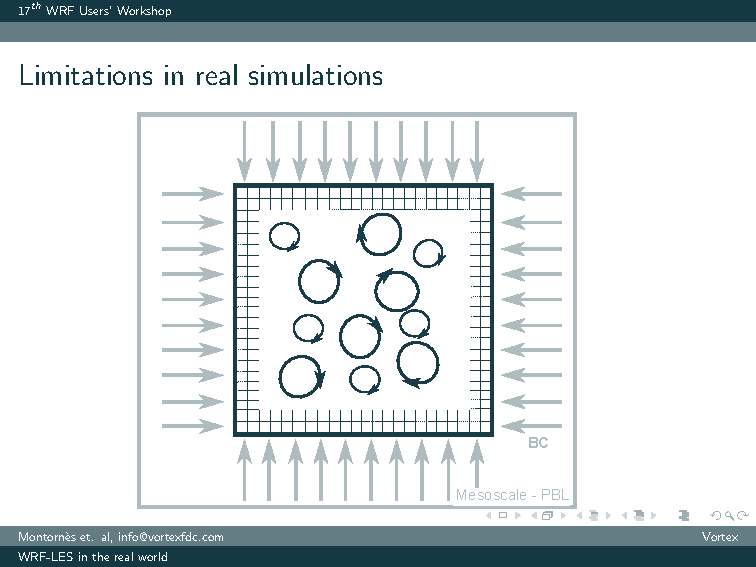
\includegraphics[width=0.4\linewidth,trim={2.67cm 1.35cm 3.1cm 2.25cm},clip]{Imagenes/02/grid}
	\caption{Idealización de los distintos tamaños de vórtices dentro de un dominio en la zona gris de la turbulencia. Los vórtices mas grandes pueden ser resueltos por la malla, mientras que los más pequeños son filtrados numéricamente y por lo tanto deben ser parametrizados para que su efecto se considere en las ecuaciones de movimiento.}
	\label{fig:02_grid_vortex}
\end{figure}

Reflexionando un poco con respecto al rol que toma la turbulencia tanto en las escalas grandes como en las pequeñas, no es difícil llegar a la conclusión que a través del proceso de escalamiento dinámico se llegará eventualmente a una zona de traslape en donde algunos de los vórtices asociados a la capa límite son indistintamente resueltos y modelados al mismo tiempo. La Figura \ref{fig:02_grid_vortex} representa este hecho. 
A esta zona de traslape se le denomina zona gris o \emph{Terra Incognita}.

Utilizando la terminología de Wyngaard (2004), sea $\Delta$ la escala (o tamaño) del filtro espacial asociado a la resolución numérica (o malla) de las ecuaciones de movimiento y $l$ la escala característica de los vórtices en el rango inercial, el espectro de energía turbulenta $\phi(\lambda)$ se ve como se muestra en la Figura \ref{fig:02_terra_inc}.

\begin{figure}[H]
	\centering
	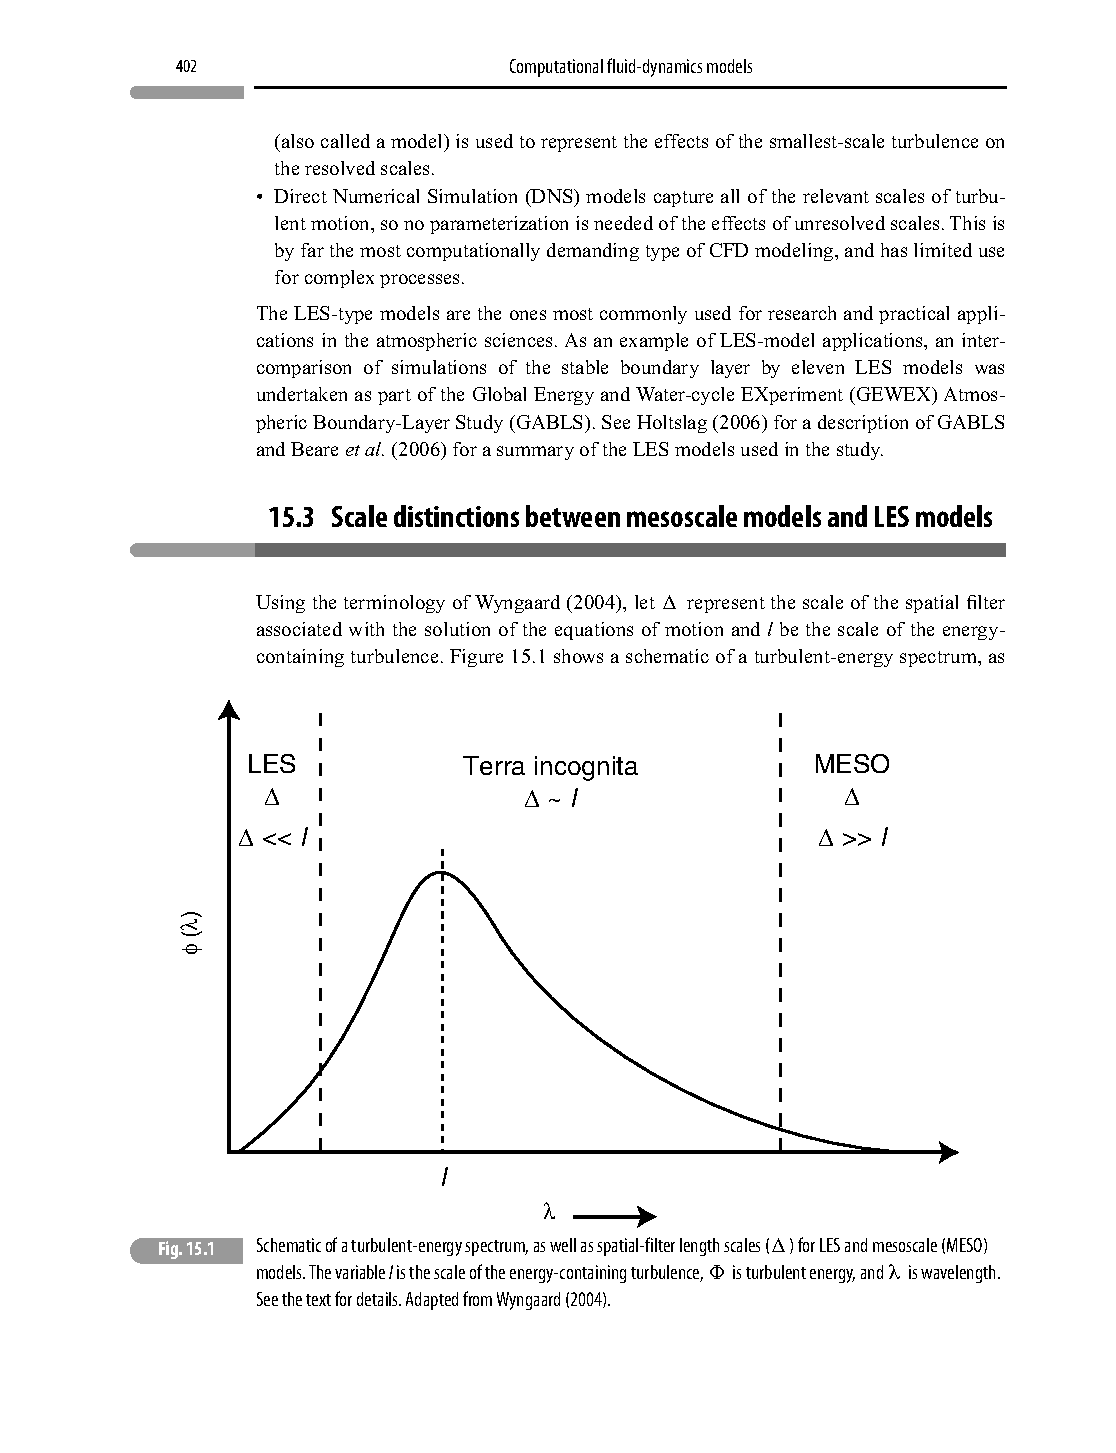
\includegraphics[width=0.69\linewidth,trim={2cm 3.0cm 1.5cm 11.5cm},clip]{Imagenes/02/terra_inc}
	\caption{Espectro de energía turbulenta multiescala.}
	\label{fig:02_terra_inc}
\end{figure}

Para valores de $\Delta\gg l$ asociados a la mesoescala, la producción de energía turbulenta queda por debajo del filtro y por lo tanto, tiene sentido que se modele a través de un esquema de submalla. Por otro lado, para valores de $\Delta\ll l$ los vórtices que contienen la energía pueden ser completamente modelado por las ecuaciones y entonces no debe usarse un SGS (microescala).

Queda entonces el rango en donde $\Delta\sim l$. Dentro de este intervalo se desconoce cual es el comportamiento de los modelos atmosféricos ya que existe una doble representación de tanto los vórtices que se resuelven como los que se modelan.

En la práctica, el acercamiento para compensar este problema es definir los dominios de modo que se evite usar el modelo en el rango de la \emph{Terra Incognita}.

\newpage
\section{Antecedentes de Modelación Turbulenta}
A continuación se presenta una breve reseña histórica de la modelación de la turbulencia atmósférica y el estado del LES.

Los primeros modelos desarrollados para poder estimar el potencial eólico parten en el año 1975, donde Jackson y Hunt presentan su análisis bidimensional para flujo turbulento en terreno complejo, el cual en 1979 fue ampliado a 3D por Mason y Stykes. Estos modelos tienen la particularidad de ser lineales y el beneficio de presentar resultados computacionalmente rápidos para pendientes no mayores a 17$^\circ$. Estos mismos modelos lineales, mejorados, actualmente se utilizan en códigos comerciales como MS3DJH, MSFD y WAsP.

En forma paralela a los modelos lineales, se fueron desarrollando métodos numéricos para resolver las ecuaciones no lineales. En 1977 Taylor desarrollo un modelo 2D no lineal de diferencias finitas para el flujo sobre una colina pequeña. Entre el 1970 y 1980 el desarrollo de algoritmos para solucionar las ecuaciones RANS fue intensivo y esto resultó en el origen de una gama de modelos de clausura para la turbulencia. El modelo clásico $k-\varepsilon$ fue originalmente propuesto en 1974 por Launder y Spalding y entre los años 80s y 90s se formularon varias modificaciones para flujos atmosféricos. En este punto, los modelos RANS presentaban una mejor solución en términos de la aceleración en la cima de las colinas y el comportamiento aguas abajo de estas.

Luego, desde los años 90s, el LES se ha estado aplicando a la capa límite planetaria para simulaciones sobre terreno plano homogéneo. El argumento a favor de la utilización del LES es que con el incremento de la potencia computacional y el refinamiento de las mallas, eventualmente se debería llegar a soluciones que sean independientes del modelo de clausura para la turbulencia. Si bien esto es teóricamente correcto, el terreno real posee rugosidad y por lo tanto se requieren modelos de pared avanzados. Estos modelos aún son dependientes del tipo de parametrización que se escoja en el método numérico.

Las simulaciones LES en terreno real entonces, se ven enfrentadas a, por lo menos, dos grandes problemas: el elevado costo computacional asociado a los tamaños de malla y el acoplamiento entre la cercanía de la pared, altamente parametrizada, con la región exterior resuelta.

A pesar de los desafíos que debe superar el LES, su potencial para modelar flujos a través de colinas ha sido altamente reconocido. Diversos autores han modelado correctamente el campo de viento en la colina Askeverin (Chow y Street, 2009; Bechmann y Sørensen 2010b) y cerros sinusoidales (Brown et al. 2001; Wan et. al. 2007), sin embargo pocos estudios en terreno complejo real existen.
\section{Alta Resolución y Terreno Complejo}
Como motivación, se comienza esta sección haciendo una pequeña derivación de la importancia de una correcta estimación de la velocidad del viento. Luego se expondrán los consensos tomados el año 2012 por el \emph{HiRCoT Workshop} (High Resolution Modelling in Complex Terrain), los cuales resumen de muy buena forma las bases y desafios actuales sobre este tema particular y que tienen especial importancia en el trabajo a desarrollar.
\subsection{Importancia de la Estimación del Viento}
Para tener un acercamiento a la importancia de la correcta estimación del viento, consideremos la energía cinética del viento. Para un área arbitraria de magnitud $A$ en un tiempo $t$ se tiene:
\begin{equation} 
E_k = \frac{1}{2}mV^2 = \frac{1}{2}(AVt\rho)V^2 = \frac{1}{2}At\rho V^3
\end{equation}

Donde $\rho$ es la densidad del aire y $V$ es la rapidez del viento. $AVt$ es entonces el volumen de aire pasando por el área $A$ que se define como normal a la dirección de la velocidad del viento $V$. La potencia del viento (energía por unidad de tiempo) para el caso de una turbina eólica queda definida entonces como:
\begin{equation}
P = \frac{E_k}{t} = \frac{1}{2}A\rho V^3
\end{equation}

Donde $A$ pasa a ser ahora el área del rotor de la turbina. La potencia del viento, es entonces, proporcional al cubo de la velocidad del viento.

Se puede derivar la ecuación anterior para hallar una relación entre los errores relativos de las dos variables de interés. Derivando la ecuación anterior se obtiene:

\begin{equation}
dP = \frac{1}{2}A\rho\cdot d(V^3) = \frac{3}{2}A\rho V^2 dV
\end{equation}

Y dividiendo ahora por la potencia eólica:
\begin{equation}
\frac{dP}{P} = 3\frac{dV}{V}
\end{equation}

Lo que significa que un error relativo (o porcentual) en una estimación de la velocidad del viento, conlleva a un error el triple mas grande para la potencia que se podría generar.

Anteriormente ya se había hablado de la relación que existe entre la complejidad del terreno y la velocidad del viento. Los fenómenos asociados a la orografía y las no linealidades provocan que la predicción del viento en estas zonas sea especialmente difícil. 

Como consecuencia, es de especial interés analizar las problemáticas que induce el terreno complejo y definir las maneras de como abordarlas.
\subsection{Problemáticas de la Simulación de Alta Resolución}
El año 2012 se llevó a cabo en Viena, el primer \emph{HiRCoT Workshop}, instancia que reunió a académicos y personas de la industria a debatir activamente sobre las problemáticas y avances existentes con respecto a la modelación atmosférica a alta resolución \cite{Arnold2010}.

El concepto de alta resolución, se debe entender en el sentido de una resolución que está por sobre aquella definida por los desarrolladores para utilizar los modelos. A priori, se podría decir que un modelo atmosférico con una resolución de malla menor a 1 [km] entra en esta categoría.

Dentro de los objetivos específicos definidos en este workshop se incluyen: la identificación de problemas asociados a la simulación numérica en terreno complejo y el mapeo de las posibilidades de como manejar estos. Por lo tanto las conclusiones emanadas de este taller sirven como buenos cimientos para este trabajo de tesis.

A continuación se presenta un resumen de los cuatro aspectos estudiados en el workshop y que se deben tener en consideración a la hora de realizar una simulación atmosférica a alta resolución y en la lectura de esta tesis.

\subsubsection{Aspecto 1: Problemas Computacionales}
Tomando en consideración que existen casos demostrados en donde la alta resolución es una necesidad para simular realísticamente fenómenos meteorológicos asociados a las escalas sinópticas y mesoescala (Morton y Molders, 2007) (Stevens et al., 2010), queda claro que, para desarrollar simulaciones a alta resolución en terreno complejo, se debe asumir un cierto compromiso computacional. El wokrshop identifica 2 temas principales: los relacionados a los tiempos de simulación y aquellos relacionados al rendimiento de I/O\footnote{Input/Output del modelo. Hace referencia al formato de los archivos de entrada y salida.} del código.

Con respecto al tiempo de simulación, se abordó el tema de como impacta en este el hecho de llevar una simulación con resolución de 9 [km] a 1 [km]. Si se mantienen los límites de los dominios numéricos constantes, el aumento en la resolución de la malla traerá consigo un aumento de la cantidad de puntos necesarios para simular. Por otro lado, este refinamiento también exigirá un paso de tiempo menor para evitar la violación de la condición CFL. En el mejor de los casos, pasar de una resolución de 9 [km] a 1 [km] en la cual la primera se demore, por ejemplo, 1 hora, implicará que la simulación a alta resolución se va a demorar aproximadamente 1 mes. Actualmente no existen maneras de reducir este aumento considerable en los tiempos de cálculo y por lo tanto pasa mas a ser un limitante en el diseño experimental. Pequeñas mejoras se pueden obtener si se adopta el uso de un paso de tiempo adaptativo, pero esto puede crear incongruencias en los tiempos de obtención de resultados del modelo, en especial para la aplicación de asimilación de datos. La paralelización de procesos también puede ayudar bastante, sin embargo para el análisis de este caso, ambas simulaciones estuvieron masivamente paralelizadas.

Con respecto al rendimiento de I/O, y que tiene especial relación con lo descrito en el párrafo anterior, el aumento en la cantidad de puntos de malla, y la disminución en el paso de tiempo, significa un aumento considerable en término de memoria para cada uno de los procesos con los que se ejecuta el código. En la arquitectura del WRF (y en la mayoría de los modelos atmosféricos) el cálculo se paraleliza en tantos procesos como procesadores se disponga utilizando un paradigma de maestro/esclavo en donde un único proceso maestro es el encargado de ejecutar las funciones de entrada/salida del modelo. A grandes rasgos el aumento de los puntos de malla no afecta tanto a los procesos que son esclavos, pero el proceso maestro si sufre de un cuello de botella al ser el encargado de leer y ubicar todas las variables globales a cada proceso. Como ejemplo académico, consideremos un dominio de 448 millones de puntos ($4000\times4000\times28$) en un servidor con 75 nodos de 4 núcleos cada uno. En este ejemplo cada proceso usará un total de 1.9GBytes, sin embargo el proceso maestro requerirá un extra de 1.8GBytes para las funciones de I/O, pudiendo ser un potencial punto de falla. En la actualidad se estan desarrollando nuevos formatos y paradigmas para facilitar la paralelización de este tipo de tareas, sin embargo una implementación de estos no se ve en el corto plazo.

\subsubsection{Aspecto 2: Problemas Numéricos}
Corresponden a las problemáticas asociadas a la discretización por la implementación de los esquemas numéricos para resolver las ecuaciones que rigen el comportamiento atmosférico. Se identificaron 5 grupos: (a) Precisión, (b) Estabilidad, (c) Difusión Numérica (explícita e implítica), (d) Sistema de Coordenadas y (f) Benchmarking.

El éxito de una simulación a alta resolución dependerá fuertemente del conocimiento de los aspectos técnicos relacionados a uso de los esquemas numéricos en el modelo a usar. Como base, la gran mayoría de los modelos atmosféricos utiliza un esquema de diferencias finitas y la integración temporal se hace de manera explícita. Esta selección en el modo de integrar numéricamente limita en gran medida la estabilidad del esquema ya que no se debe violar la condición CFL. La implementación de un esquema implícito permite ganar estabilidad, en el sentido de la condición CFL, sin embargo las numéricas se complejizan y la resolución implica ahora solucionar una ecuación elíptica la cual es difícil de paralelizar en super computadores.

La presencia de terreno complejo, por otra parte, incentiva la aparición de ruido numérico debido al desarrollo de perturbaciones de alta frecuencia las cuales desafían la precisión del esquema de advección, los gradientes de presión y la consistencia de los términos métricos. Para evitar esto se suele suavizar el terreno, aunque para el caso de una simulación a alta resolución esto no es deseable ya que se pierde una parte sustancial de la fineza del terreno, que es lo que se quería ganar en primer lugar. 

A continuación se revisan los aspectos mas relevantes de cada grupo relacionado con las numéricas del problema.

\paragraph{Precisión} Se entiende como precisión, el orden con el cual se reducen los errores de truncación debido a un refinamiento temporal o espacial. Mejores esquemas numéricos implican una mejor precisión, sin embargo son mas costosos computacionalmente. Para simulaciones a alta resolución en terreno complejo, los datos utilizados para inicializar el modelo ya vienen con una resolución propia de los instrumentos de medición usados. Estos datos pueden ensuciar la precisión formal que tenga un cierto esquema numérico debido a que los errores inducidos por los datos predominaran por sobre aquellos del modelo. De ahí que para este tipo de simulaciones, la utilización de esquemas de alto orden no se presenta como un beneficio tan tangible.

\paragraph{Estabilidad} Como se habló anteriormente, debido a la predominancia de los esquemas explícitos, los modelos de NWP están sujetos a criterios de estabilidad numérica. El primer criterio es el CFL, asociado a la advección, donde se debe cumplir que:
\begin{equation}\label{eq:cfl}
\frac{u\Delta t}{\Delta x}<\beta_a
\end{equation}
Donde $u$ es una la rapidez de propagación física de alguna señal y $\beta_a$ es un coeficiente que depende de la discretización. El otro criterio importante es el asociado a la difusión, el cual se escribe como:
\begin{equation}\label{eq:cfl_d}
\frac{\nu\Delta t}{\Delta x^2}<\beta_d
\end{equation}
Acá $\nu$ es un coeficiente de difusión y $\beta_d$ es otro coeficiente que depende de la discretización. Notar que en este segundo criterio, el valor escala de manera cuadrática con $\Delta x$, lo que implica que $\Delta t$ deberá disminuir proporcionalmente a $\Delta x^2$ para mantener estable la integración de los términos difusivos. En simulaciones estándar, el común usar un coeficiente de difusión que escale según $\Delta x^2$ (Smagorinsky por ejemplo), luego este criterio es mas vulnerable a ser violado a muy alta resolución.

Algunas técnicas prácticas que se utilizan para evitar las inestabilidades incluyen el uso de pasos de tiempo adaptativos que impidan el no cumplimiento de los criterios antes mencionados o el uso de amortiguamiento para la componente $w$ de la velocidad, que es la mas crítica en la simulación de terreno complejo. El uso de amortiguamiento genera soluciones no físicas y por lo tanto no está bien visto por la comunidad científica.

\paragraph{Difusión Numérica} La difusión artificial (o numérica) o disipación artificial es la amortiguación sucesiva de perturbaciones como consecuencia de las propiedades del método numérico. De la misma manera en la que actúa la difusión física, las variaciones de las escalas pequeñas se tienden a suavizar. Esto puede ser provocado implícitamente debido a la diferenciación espacial o explícitamente como un término en las ecuaciones resueltas. Este es un fenómeno complejo y generalmente el manejo de este se encarga a los diseñadores de los núcleos dinámicos de los modelos. A nivel de usuario, una regla práctica es saber que aquellos esquemas espaciales que son de orden par poseen una mayor difusión que aquellos de orden impar, por ende se prefiere el uso de estos últimos.

La difusión artificial posee algunos aspectos positivos, puede mantener bajo control el ruido numérico que se provoca a pequeñas escalas, sin embargo, si existe mucha difusión numérica toda una simulación realizada a alta resolución puede verse suavizada debido al efecto de esta y podría no rescatarse el comportamiento debido al terreno complejo.

Para ámbitos operativos, se prefiere no utilizar difusión horizontal explícita o realizarla solo en coordenadas reales. La difusión implicita es mas dificil de controlar, pero esta no afecta de gran manera al comportamiento sobre terreno complejo a no ser para grandes magnitudes del viento. 
\paragraph{Coordenadas} Para solucionar las ecuaciones que gobiernan el comportamiento atmosférico, los modelos NWP utilizan sistemas coordenados no necesariamente Cartesianos. La mayoría de los modelos utiliza sistemas que persiguen la forma del terreno, entre los que se pueden nombrar:
\begin{itemize*}
	\item Coordenadas ``sigma'' de presión o coordenadas de altura.
	\item Coordenadas curvilíneas adaptadas al borde.
	\item Coordenadas Cartesianas con el método de frontera inmersa.
\end{itemize*}

 
\begin{figure}[h!]
	\centering
	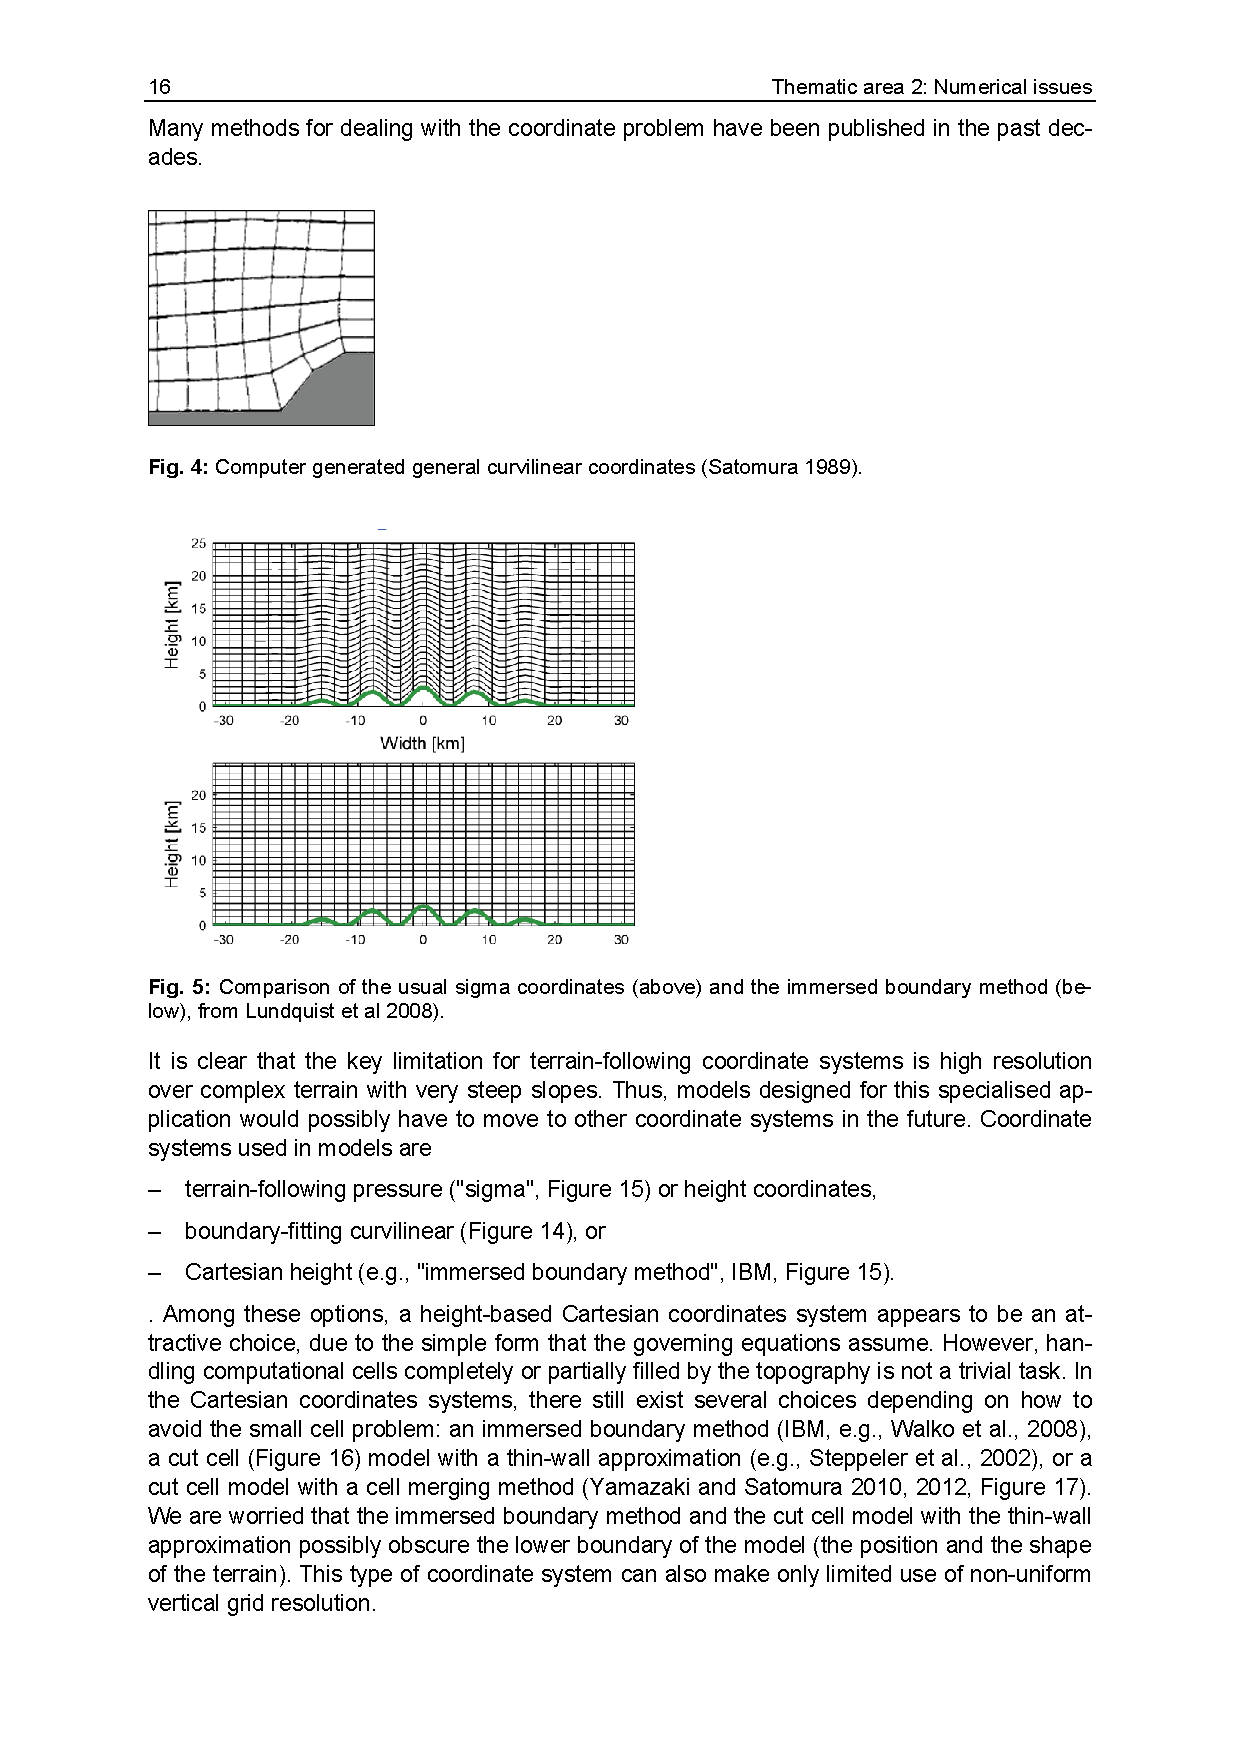
\includegraphics[width=0.8\linewidth,trim={2.6cm 13.5cm 9.2cm 9cm},clip]{Imagenes/02/coordinates}
	\caption{Comparación entre las coordenadas usuales sigma (arriba) y el método de frontera inmersa (abajo).}
	\label{fig:02_coordinates}
\end{figure}
La transformación de coordenadas naturales a curvilíneas provoca en las ecuaciones gobernantes la aparición de términos métricos, los cuales son difíciles de manejar en pendientes abruptas, pero permite captar bien la forma del terreno. Por otra parte el uso del método de la frontera inmersa no incluye cambio en las ecuaciones pero el manejo de las celdas que están parcialmente ocupadas por orografía no es una tarea computacional sencilla.

Si bien, para cualquiera de estos dos casos existen problemáticas computacionales que no son fáciles de solucionar, la más limitante en la actualidad es el manejo de las pendientes abruptas y la exigencia que esto significa en la resolución de malla vertical y la aritmética de grandes diferencias de presión. Por lo tanto, el pronóstico de la comunidad, es a migrar a un sistema coordenado cartesiano utilizando el método de frontera inmersa u otros métodos similares en la cercanía del terreno, como la aproximación de pared delgada (Steppeler et. al., 2002) o el método de unión de celdas (Yamazaki y Satomura 2010,2012).

\paragraph{Benchmarking} La existencia de benchmarks (casos de comparación) es clave para este tipo de simulaciones. Lo que se posee actualmente son casos ideales de colinas gausianas para el estudio de ondas de montañas, casos en donde se poseen soluciones analíticas para comparar. Este tipo de casos se justifica actualmente solo en contextos muy simples y por lo tanto se está llevando a cabo el esfuerzo de generar una mayor cantidad de casos y datos para comparar que tengan relación con el terreno complejo a alta resolución. Lo que se espera en el futuro incluye:
\begin{itemize*}
	\item Casos reales donde se posean una gran cantidad de observaciones tridimensionales a alta resolución.
	\item Integración temporal a largo plazo para casos reales que puedan ser usados para revisiones estadísticas.
	\item Además del flujo medio, tener información sobre las variables de segundo orden tales como los flujos de momentum y radiación.
\end{itemize*} 
\subsubsection{Aspecto 3: Parametrizaciones de Capa Límite}
Los fenómenos asociados a la capa límite y a la mezcla a nivel de superficie son generalmente parametrizados en base al conocimiento de la turbulencia homogénea en terreno plano (por ejemplo, la teoría de similaridad) y bajo condiciones óptimas (estratificación cuasi-estable). Estas condiciones no son las que se encuentran en terreno complejo. Las parametrizaciones clásicas de capa límite funcionan bien hasta mallas del orden de los kilómetros, bajo este rango su aplicación se torna cuestionable (zona gris).

Con respecto a la alta resolución de la malla, los modelos numéricos actuales utilizan dos acercamientos para resolver la turbulencia:
\begin{enumerate*}
	\item[a.] \emph{Promedio de Ensamble}: Las ecuaciones de Navier-Stokes son descompuestas en una componente media y una componente fluctuante (descomposición de Reynolds). La turbulencia queda completamente parametrizada en función de las variables del flujo medio (en la llamada parametrización de capa límite). Por definición, todas las variables del modelo son valores promedios.
	\item[b.] \emph{Large Eddy Simulation}: En esta, las ecuaciones de Navier-Stokes son filtradas con un largo del filtro ubicado dentro del rango inercial del espectro turbulento. De esta manera, el modelo resuelve solamente los grandes vórtices y la turbulencia de pequeña escala, considerada isotrópica, es parametrizada. Las variables de salida de un modelo LES son, en principio, instantáneas, pertenecientes a una realización específica de un proceso aleatorio.
\end{enumerate*} 

Convenientemente, las ecuaciones pronósticas del flujo medio atmosférico para estos dos acercamientos son, idénticos. La diferencia radica en el detalle en como se obtiene la clausura del término turbulento.

Uno de los problemas relevantes, es que la parametrización usual para el promedio de Reynolds es unidimensional, en el sentido que solamente considera los flujos turbulentos verticales, calculados en función de las condiciones de una sola columna en la malla; mientras que para terreno complejo, las estructuras turbulentas son completamente tridimensionales. A medida que la malla se va volviendo mas pequeña, los flujos turbulentos horizontales y la advección de energía cinética turbulenta (en adelante TKE) se va volviendo mas importante y además se vuelve cuestionable el conocimiento de las estructuras turbulentas que son efectivamente parametrizadas y las que son efectivamente resueltas. 

En los dominios del LES (mallas bajo el kiómetro), los flujos turbulentos relacionados a los grandes vórtices y la producción de TKE comienzan a ser explícitamente resueltos. En esta zona, el LES ha sido raramente probado en terreno complejo y además aún presenta varios problemas abiertos. Considerando el acercamiento usual de utilizar dominios anidados para obtener condiciones de borde realistas, un dominio pequeño LES debe estar anidado a otro mas grande sin LES. La unificación de estos dos dominios no es una tarea sencilla ya que presenta una serie de problemas, entre ellos: (a) el ruido generado en los bordes del dominio anidado, (b) el \emph{spin-up} necesario para que el dominio LES represente adecuadametne la turbulencia, y (c) el tamaño de los dominios de tal forma que los efectos de borde queden fuera de la región de interés.

Junto con esto, se debe tener en cuenta también que, el conocimiento actual sobre la turbulencia en terreno complejo (i.e. las características que el modelo numérico debiese reproducir) es bien limitado y por lo tanto todos los desarrollos en aspectos numéricos deben ir de la mano con esfuerzos experimentales para obtener mejores observaciones.

Todo lo antes expuesto demuestra que, la utilización de LES en terreno complejo es un tema popular y de interés para la comunidad de modelación atmosférica.

Con respecto a la interacción entre las parametrizaciones de capa límite y los procesos de superficie, se han identificado las siguientes problemáticas:
\begin{enumerate*}
	\item[a.] Radiación: Es necesario modificar los modelos para considerar los efectos de las pendientes y de las sombras en topología compleja, en especial para las simulaciones a alta resolución. Si bien, la implementación de estos algoritmos son simples, la utilización en sistemas en paralelo se complica debido a que se necesita el cálculo de efectos de sombra no locales que en mallas muy finas pueden significar una gran cantidad de puntos.
	\item[b.] Validez de la teoría de Monin-Obukhov: La teoría de similaridad se genera en base a información en terreno plano y homogéneo, y, a priori, no se conoce hasta que punto puede ser aplicada a terreno complejo. Se discuten dos problemáticas de esto: (i) la suposición de homogeneidad horizontal (la cual, para simulación a muy alta resolución no debiese ser el problema dominante) y (ii) el intercambio de momemtum: la mayoría de los modelos parametrizan el intercambio de momemtum solamente en función del esfuerzo de corte. De manera general, un buen modelo de superficie debiese tomar en consideración la tridimensionalidad y la heterogeneidad espacial de la turbulencia en terreno complejo.
	\item[c.] Albedo, Nieve, Humedad del Suelo: Estos parámetros son muy importantes para flujos inducidos térmicamente, energía y balance de agua. Los modelos de suelo generalmente son unidimensionales, pero en terrenos montañosos es necesario  que sean bi o tridimensionales. También, debe ser necesario un acoplamiento entre el modelo atmosférico  y modelos hidrográficos o de nieve para tener resultados correctos. 
	\item[d.] Desviación de Viento Superficial: Los modelos generan magnitudes para el viento en la superficie demasiado elevadas para terreno plano y valles, debido a que la topografía de submalla no resuelta causa esfuerzos superficiales que no son representados. Varios modelos solucionan esto agregando un término de esfuerzo o aumentando el largo de rugosidad, dependiendo de la varianza de la elevación de submalla. El primero de estos métodos es recomendado debido a que cambiar la longitud de rugosidad tiene efectos colaterales en los flujos de calor y humedad.
	\item[e.] Arrastre por Ondas de Gravedad: En terrenos montañosos, el arrastre por ondas de gravedad, representan una componente importante del flujo de momemtum de submalla para las corrientes en jet. En los modelos, para que esto se considere, deben ser tomados en cuenta los efectos direccionales de submalla.
\end{enumerate*}

Finalmente, los esfuerzos para los futuros avances en las parametrizaciones de capa límite, que serán aquellos que se utilizarán en los modelos de la próxima generación, iran enfocados en las siguientes lineas:
\begin{enumerate*}
	\item[a.] Modificaciones a los Esquemas Existentes: Básicamente incorporar variables que hasta ahora no han sido consideradas, como por ejemplo la velocidad vertical para los modelos de microfísicas y considerar una dependencia explícita de la altura, entre otros.
	\item[b.] Esquemas Nuevos: Aún se necesita el desarrollo de esquemas nuevos, por ejemplo: parametrizaciones de submalla para efectos de microescala en circulaciones locales, turbulencia y pulsaciones en rotores, y tormentas cuesta abajo.
	\item[c.] Efecto de la Orografía de Submalla: Para reducir las desviaciones de los perfiles de viento.
	\item[d.] Parametrizaciones de Submalla para Modelos de Escala Gruesa.
\end{enumerate*}

\subsubsection{Aspecto 4: Inicialización y Datos de Entrada}
Todos los modelos atmosféricos requieren condiciones iniciales superficiales y atmosféricas, además de condiciones de borde laterales e información estática para los dominios de simulación. Las condiciones iniciales y de borde generalmente vienen dadas por un modelo global. La información estática caracteriza las propiedades y el estado de la superficie, como lo es: la topografía, el albedo, la categoría de uso de suelo, la fracción de vegetación y la textura del suelo.

La información estática nativa de los modelos estándar tiene a lo más una resolución de 1 [km], por ende, para lograr una correcta simulación a alta resolución y en terreno complejo, es necesario alimentar al modelo con bases de datos de alta resolución.

Para las bases de datos orográficas, debido al peso de las bases de datos, los modelos vienen por defecto con información de a lo más 1 [km] de resolución, como lo es por ejemplo el GTOPO30 USGS (información a 30'' de resolución). Para alcanzar la alta resolución se deben incorporar nuevas bases de datos. Existe información disponible desde la \emph{Shuttle Radar Topography Mission} (SRTM) con 3'' (100 [m]) de resolución y tambien de ASTER (\emph{Advanced Spaceborne Thermal Emission and Reflection Radiometer}) con 1'' (30[m]) de resolución. El problema en ambos es el terreno complejo donde algunas veces hay errores (sombras, cálculo de topografía). Algunas veces, existe información nacional obtenida con escáner laser, pero generalmente no están abiertas libremente. Finalmente, la incorporación de las bases de datos de alta resolución a los modelos atmosféricos no es directa ni sencilla y la instalación de estas puede generar nuevos problemas.

Con respecto a la información de la superficie del suelo, las bases de datos usuales, por ejemplo la data de USGS (1 [km]), es de los 90s y por lo tanto está desactualizada al no considerar el cambio en la vegetación y la deforestación. Nuevas bases de información, por ejemplo MODIS o CORINE (3'') usan 20 clases para clasificar el suelo, el cual es un número bajo de categorías como para caracterizar el terreno, además estas son locales y no globales. La información de la superficie del suelo se utiliza para calcular, entre otros, el albedo, el largo de rugosidad y la vegetación en cada punto de malla. Esta información se puede obtener también de estudios regionales o modelos agro-meteorológicos, sin embargos estos no se adecuan a algún estándar en específico y su incorporación es tediosa.
 
Para las condiciones iniciales del modelo, tener información adecuada es una precondición para generar simulaciones de mesoescala a alta calidad. Generalmente, estas condiciones las provee un modelo operativo global (sinóptico) el cual, por definición, no posee condiciones de borde. Luego, la información de ese modelo debe ser escalada a la malla del modelo mesoescala. Además, dentro de la misma simulación de mesoescala, los campos de los dominios exteriores deben ser escalados en los bordes de los dominios interiores (\emph{nesting}). El escalamiento (o interpolación) se requiere tanto espacial como temporalmente. Los modelos globales utilizan pasos de tiempo típicos de 15 [min], sin embargo el estándar es entregar los resultados en intervalos horarios, por ejemplo 3 [h]. Los modelos mesoescala utilizan pasos de tiempo del orden de los 5 [min] y mucho menor para simulaciones de alta resolución. Las condiciones de borde laterales son creadas entonces por interpolación de los outputs del modelo global (cada 3 horas) a cada 5 minutos generando una serie de tiempo. Debido a la naturaleza de las condiciones, es claro que estas no contienen información física relevante en escalas de tiempo menor a las 3 horas, por lo tanto se deben aplicar un par de medidas cuando se trabaja para dominios donde son relevantes las pequeñas escalas: (i) utilizar una zona de buffer de manera que que los bordes laterales estén lejos de la zona de interés meteorológico y (ii) evitar grandes forzamientos orográficos en los bordes, por lo tanto se deben posicionar los bordes de los dominios en zonas alejadas de terreno complejo. 

A continuación  se listan algunas fuentes de información libres que proveen bases de datos como las descritas anteriormente:
\begin{itemize*}
	\item ASTER GDEM
	\item STRM data
	\item GlobCover 2009
	\item GlobCarbon 2007
	\item MODIS
	\item FAO
	\item HWSD 2009
	\item ESDB
	\item ECOCLIMAP-2
	\item LSA SAF
\end{itemize*}
\newpage
\section{Uso Operativo de Asimilación de Datos}
La asimilación de datos es el proceso mediante el cual se busca la mejor  estimación del estado de la atmósfera a través de una combinación lineal entre un conjunto de observaciones y el resultado de un modelo. A esta estimación se le llama análisis.

Actualmente la asimilación de datos es ampliamente utilizada para corregir las desviaciones propias de las simulaciones de la dinámica atmosférica para los casos de las escalas globales y sinópticas, ya que para ese rango existen una gran cantidad de datos de acceso libre que se pueden utilizar. Los resultados para los casos de gran escala han sido satisfactorios y por lo tanto el uso de la asimilación de datos se ha tornado cotidiano sin mayores cuestionamientos.

Para el caso de la asimilación en la capa límite, las investigaciones son escasas y en muchos casos, poco concluyentes. Se pueden resumir las investigaciones en esta área en tres grupos: (i) Incorporación de asimilación de datos en la capa límite planetaria en grandes escalas, (ii) Asimilación de datos de información superficial y (iii) Asimilación de datos en la PBL en la microescala. 

Para el primer grupo, se pueden mencionar las investigaciones de Cheng et al. (2017) \cite{cheng2017short} y Dumais et al. (2013) \cite{dumais2013implementation}. Acá efectivamente se asimilan datos dentro de la capa límite, pero en dominios de mesoescala, lo que significa que se puede acceder a una gran cantidad de punto, como por ejemplo, en el primer artículo donde se tiene la información de los anemómetros de las turbinas de varios parques. Dentro de este grupo también se ubican investigaciones que tienen relación con el ámbito militar y por lo tanto muchos resultados no son públicos. Las conclusiones de estos trabajos muestran mejoras de hasta un 30\% para el error en la magnitud del viento.

En el segundo grupo se ubican las investigaciones de Stauffer et al. (1991) \cite{doi:10.1175/1520-0493(1991)119<0734:UOFDDA>2.0.CO;2} y  Reen y Stauffer (2010) \cite{reen2010data}. En estas, lo que se asimila son las variables de la superficie, como por ejemplo: la temperatura del suelo o la humedad. Esta información es sencilla de obtener si se hacen campañas de medición con radiosondas. Luego, es posible obtener una alta densidad de datos en un terreno localizado. Los resultados de estos casos han demostrado que existe una mejora al asimilar datos superficiales, ya que se predice de mejor manera los flujos turbulentos superficiales.

Con respecto al último grupo, son casi inexistentes las investigaciones debido a dos motivos: (a) De por si son pocos los trabajos de simulación multiescala en donde se llegue a dominios con tan alta resolución y por ende, la mayoría de esos trabajos va mas enfocado a mejorar el LES que a la implementación de otros procesos numéricos, y (b) Para tener un buen resultado de la asimilación de datos es necesario poseer una alta densidad de puntos, la cual, a escalas muy localizadas no es posible obtener sin hacer uso de algún tipo de instrumentación especial o alguna red de medición experimental que lo permita. Con respecto a esto último, se tiene conocimiento de varios trabajos en universidades extranjeras que se enfocan en el desarrollo de redes multisensoriales para evaluar el recurso eólico en zonas localizadas, sin embargo la información de esos proyectos es privada y de desconoce el resultado de la asimilación de datos para estos casos.

La aplicación de la asimilación en la ABL generalmente se ha dejado de lado debido a que, de por si, las predicciones para la magnitud del viento aún presentan grandes discrepancias con las mediciones en terreno y por lo tanto, asimilar datos puede que sea mas perjudicial que benéfico. Así, la mayoría de lo esfuerzos académicos han estado en el desarrollo de parametrizaciones de PBL mas precisas. 

Finalmente, las investigaciones relacionadas a la interacción entre la asimilación de datos y el terreno complejo, por ejemplo Hacker et al. (2018) \cite{hacker2018challenges}, han ido mas en el enfoque de hallar relaciones entre las variables superficiales y el comportamiento de la atmósfera, mas que la incorporación de datos en la ABL. Hay evidencia que, en terreno complejo, el comportamiento del viento está mas desincronizado de las variables superficiales que el terreno plano y por lo tanto la asimilación de datos de estas es menos efectiva.
\newpage
\section{Síntesis}
A modo de destacar las ideas fundamentales que se presentaron en este capítulo, a continuación se muestra un listado de los argumentos que hacen que la investigación a realizar sea académicamente atractiva:
\begin{enumerate*}
	\item No existen casos documentados en donde se haya exigido al modelo WRF una resolución tan alta como 2 [m] en terreno real con LES.
	\item El terreno a simular es complejo y por lo tanto se expondrá la interacción del LES con este.
	\item Se pondrán a prueba las bases de datos de alta resolución que sean de carácter públicas y libres.
	\item Se hará de manera efectiva un proceso de asimilación de datos a nivel de capa límite en un dominio de microescala.
	\item Los resultados obtenidos servirán como benchmark para futuras investigaciones.
\end{enumerate*}

Finalmente, y parafraseando al académico Charles Menevau (2019) \cite{doi:10.1080/14685248.2019.1584664}, la aplicación de métodos como la asimilación de datos dentro de la capa límite planetaria sigue siendo un área activa y atractiva de investigación. La descarbonización de la matriz energética mundial exige nuevos estándares para la predicción relacionada a energías renovables, y en el caso de la energía eólica, el núcleo del problema de la predicción yace en la física fundamental de la respuesta de la turbulencia de pared al forzamiento transiente de las grandes escalas.

